\pdfoutput=1
\documentclass[11pt]{article}

\usepackage{graphicx}
\usepackage[space]{grffile}
\usepackage{latexsym}
\usepackage{textcomp}
\usepackage{longtable}
\usepackage{multirow,booktabs}
\usepackage{amsfonts,amsmath,amssymb}
\usepackage{url}
\usepackage{hyperref}
\hypersetup{colorlinks=false,pdfborder={0 0 0}}
% You can conditionalize code for latexml or normal latex using this.
\newif\iflatexml\latexmlfalse
\usepackage[utf8]{inputenc}
\usepackage[english]{babel}

\usepackage{setspace}
\usepackage{apacite}
\usepackage[margin=1in]{geometry}



\begin{document}

\title{Analysis of Dyadic Interaction in an Interview Setting}

 \author{Suresh Alse, Bhavishya Sharma, Jay Priyadarshi, Abhishek Sharma}

\maketitle




\nocite{*}
\section{Introduction}
Interviews are often hard to be judged. It is often left in the hands of the interviewer(s) to measure the hirability of the candidates. This is fundamentally flawed as this heavily relies of interviewers' mood and personality. Also, in most cases multiple interviewers interview for the same roles which makes this process even less scientific as it is almost impossible to fairly aggregate the opinions of interviewers.

There has been tons of research by psychologists and career experts about what one should do in order to succeed in an interview \cite{huffcutt2001identification}. From this, we know that things like smiling, using a confident tone and making good eye contact can contribute a lot in an interview. However, these observations are often based on intuition and experience. Hence, It is hard to automate and quantify hirability of candidates. Also, there is a common misconception that content of the interviewee's responses is the sole determinant of the job interview. However, it is seen that non verbal aspects are as important if not more important than verbal responses \cite{mehrabian1971silent}.

\begin{figure}[h!]
\begin{center}
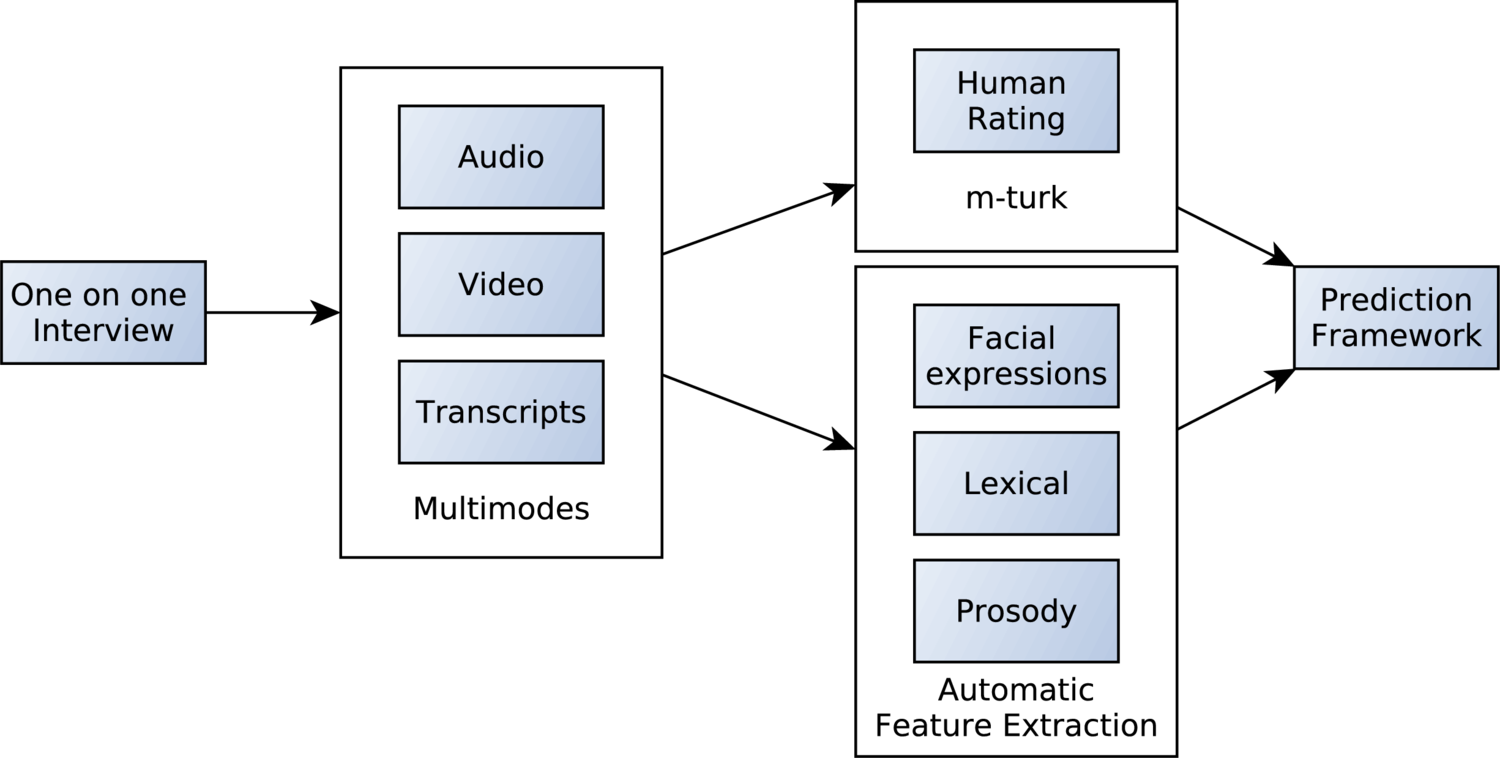
\includegraphics[width=0.7\columnwidth]{figures/process1/process1}
\caption{{Proposed Framework%
}}
\end{center}
\end{figure}

In this project we would like to build a computational framework using which interviewers and interviewees can use it to analyze interviews and obtain the following.
\begin{itemize}
\item Automatically predict the overall score of the interview.
\item Quantify verbal and nonverbal behavior of the interviewee towards the success in the interview.
\item Automatically recommend aspects to be improved for better overall score. 
\item Timeline that shows how well the interview progressed with respect to time.
\end{itemize}

In order to achieve this we propose a framework as shown in the figure below. We use a one on one interview data comprised of three modes (audio, video and textual). Then, we extract multimodal features (facial expressions, lexical and prosody) and predict the overall score of the interview, how likely the candidate is going to be hired and other traits required for the interview process.


\section{Related Work}
A lot of the research in the field of mulitmodal analysis of interaction has focused on speech and visual analysis of data. For instance, in Rough'n'Ready: A Meeting Recorder and Browser \cite{kubala1999rough}, they provide a way to recognize speech in the form of a BBN Byblos Speech Recognition System, where they also provide a mechanism to browse and retrieve speech data with the help of a speech index. Speaker identification is also described in The Meeting Project at ICSI \cite{morgan2001meeting}, where the acoustic model consisted of gender-dependent, bottom-up clustered (genonic) Gaussian mixtures. Further, leveraging speech recognition, topic detection in a meeting room scenario is described in Advances in Automatic Meeting Record Creation and Access, where they use a variant of Hearst's TextTiling algorithm in order to automaticaly segment the transcript into topically coherent passages.

As far as visual analysis is concerned, we can find examples of that in SMaRT: The Smart Meeting Room Task at ISL \cite{waibel2003smart}, where they provide a mechanism to track people and identify them as they move around a Meeting Room using multiple cameras and advanced computer vision techniques. Another good example of that would be Distributed Meetings: A Meeting Capture and Broadcasting System \cite{cutler2002distributed} where they augment the meeting room for remote viewers by adding cameras and other functionalities.

A major focus on such speech and visual processing (as provided above) has been focused on individuals, however, even when the researchers examine a meeting space. Our aim is to analyze dyadic communication where we don't just monitor an individual, but we attempt to find multimodal cues (such as back-channels among others) which would then uncover the underlying mechanism of a job interview.

There has been research on analyzing behavior of a group as compared to an individual, as is exemplified by research like The KidsRoom: A Perceptually-Based Interactive \cite{bobick1999kidsroom} and Immersive Story Environment and A Bayesian Computer Vision System for Modeling Human Interactions \cite{oliver2000bayesian}. However, the research here focuses on problem specific "primitive tasks", and therefore involves a much more constrained examination, which is in a sharp contrast to a sort of free-flowing, spontaneous (dyadic) interaction that we would have hoped for.

While our system focuses on some form of speech and visual processing, and also incorporates analysis of dyadic interaction as a whole, we provide a way to analyze the interaction in a much more unconstrained manner, identifying key multimodal cues, unraveling the underlying operating factors of a job interview by treating an interview as "more than a some of its parts" and hopefully, to come up with capabilities to automatically predict the overall score of an interview, quantify verbal and non verbal behavior of the interviewee towards the success in the interview, automatically recommend aspects to be improved for a better overall score, and a timeline to show how well an interview progressed with respect to time.

\section{Dataset}
We use the MIT Interview Dataset \cite{naim2015automated} for this project that we obtained by contacting the authors of the project. It consists of 138 recordings of mock interviews of students from MIT, seeking internships. The interviews were conducted in a one on one interview fashion. Both interviewers and interviewees were equipped with microphones which allows us to extract and differentiate between the speakers easily. Cameras were used to capture the video of the interviewee during the process as shown in the Figure \ref{fig:dataset}. The interviews were conducted by two professional career counselors with over five years of interviewing experience. All participants are native english speakers (this is very important because in our approach things like confidence, fluency, etc are considered). For every participant, two rounds were conducted - before and after intervention. Overall, 69 students permitted the use of recordings for research purposes. Hence we have a total of 138 recordings of lengths between 3 minutes to 8 minutes (average: 4.7 minutes per interview). Every interview consisted of interviewer asking the interviewee, five questions and no job description was given to the interviewees. The researchers who collected this data claim that this is the largest collection of job interview videos conductedby professionals.

To rate the interview, Amazon mechanical turk workers were used. Each turker watched the interview videos and rated the interviews by answering 16 assessment questions \ref{tab:assess} on seven point scale. Questions about ``Overall rating'' and ``Recommend Hiring'' captures overall score where as other questions capture higher level behavior. 
\begin{table}[h!]
    \centering
    \begin{tabular}{ | c | }
	\hline
        Engagement \\
	\hline
        Excited \\
        \hline
        Friendly \\
        \hline
        Smiled \\
        \hline
        NoFillers\\
        \hline
        RecommendedHiring \\
        \hline
        Overall \\
        \hline
        EyeContact\\
        \hline
        NotAwkward\\
        \hline
        StructuredAnswers\\
        \hline
        Calm \\
        \hline
        Focused\\
        \hline
        NotStressed\\
        \hline
        Authentic\\
        \hline
        Paused \\
        \hline
        SpeakingRate\\
        \hline
    \end{tabular} 
    \caption{Assessment questions}
    \label{tab:assess}
\end{table}

The dataset also consists of transcripts of all the interviews. This was made possible by Amazon mechanical turk workers hired by the researchers. Also, they were instructed to include filler words such as ``like'', ``uh'', ``umm'' along with cues like ``[long pause]'', ``[smiling]'' etc which are very useful for our process.

We also tried semaine-db \cite{mckeown2012semaine} which seemed good for this project. However, it just consisted data of two individuals talking to each other and was in no way an interview setting. We also considered using AMI database which consisted of a group discussing about a particular topic for a day. However, this had additional problems such as multiple people in a frame, etc and moreover similar to semaine-db, this was not a interview setting. Also, as this needs a considerable amount of data in a given setting and then requires amazon mechanical turkers, creating our own dataset seemed farfetched. Hence, we chose MIT Interview Dataset which is perfect for our project. 

\begin{figure}[h!]
\begin{center}
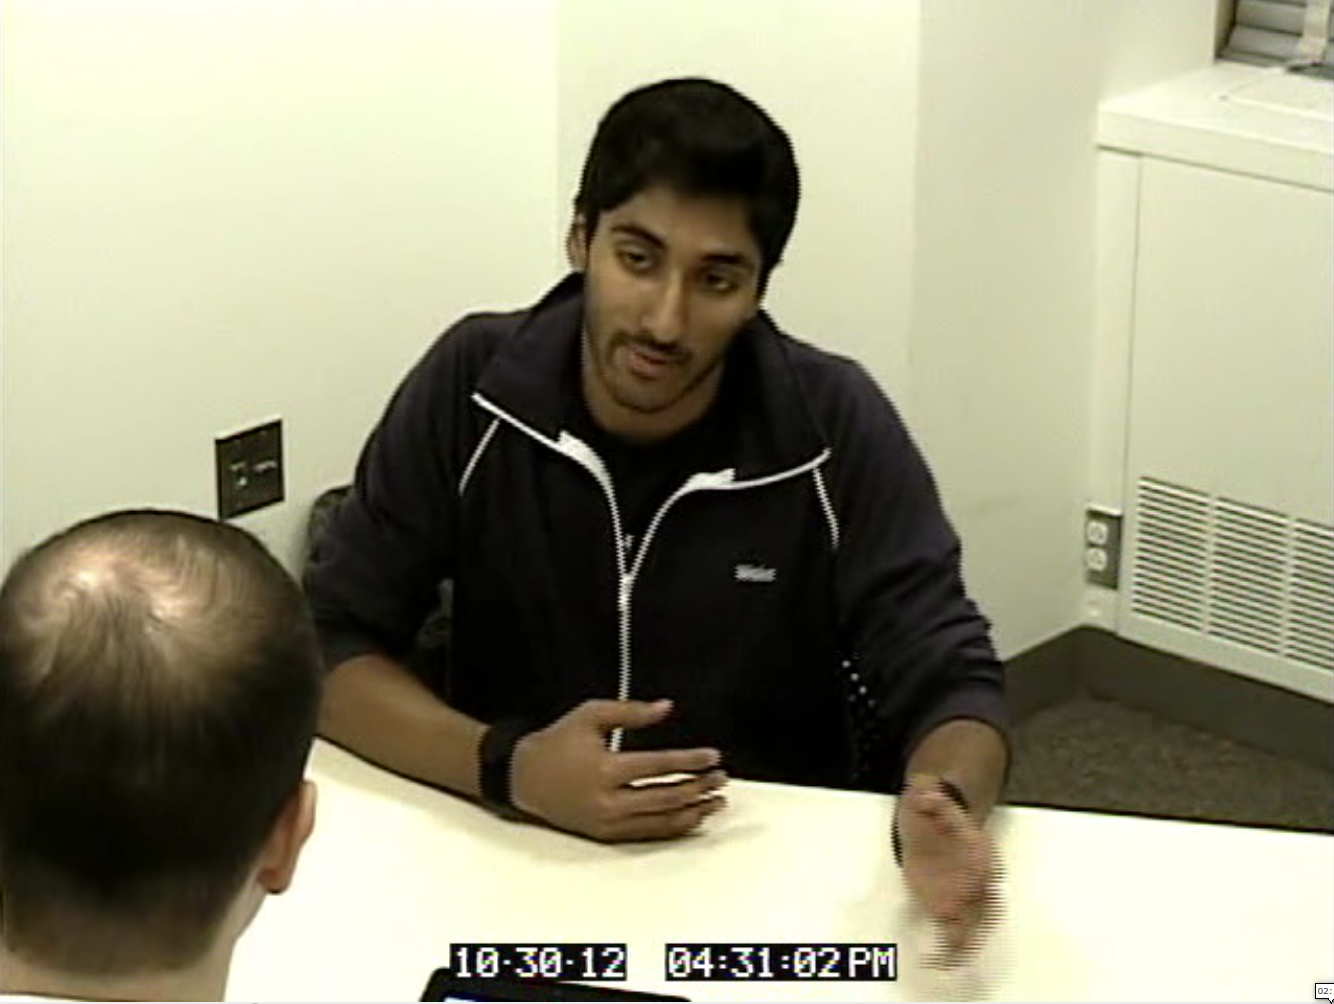
\includegraphics[width=0.7\columnwidth]{figures/Screenshot from 2016-10-21 20-30-05/Screenshot from 2016-10-21 20-30-05}
\caption{One of the 138 interviews.}
\label{fig:dataset}
\end{center}
\end{figure}

\section{Methodology}
This section we describe the overall approach towards building the proposed framework.
\subsection{Feature Extraction}
We consider three categories of features in our approach i.e Prosodic features, lexical features and facial features. Also, as the data provides with necessary transcripts from m-turkers along with filler words, we don't have to use any automatic speech recognition. Hence lexical features can be extracted directly from transcripts.
\subsubsection{Prosodic Features}
In order to extract prosodic features from the audio, we are planning to use an open source speech analysis tool called PRAAT \cite{naim2015automated}. We obtain the features from parts where interviewer and interviewee speak separately. We then obtain averages over every response and over five responses. Thus we can both reduce dimensionality and retain temporal nature of the prosody that is required for our analysis.

According to some of the previous research \cite{frick1985communicating}, pitch, intensity, characters of first three formants and spectral energy are found to be more representative of our behavior. For every feature we extracted mean, variance, minimum and maximum values. We also extracted additional features such as pauses, non-uniform pitch and intensity of speeches as it will help in determining overall score of the interview.
\subsubsection{Lexical Features}
Word count is often used as lexical feature in many applications. However, we only have limited data; hence, we will not be able to use it as it would result in sparse high dimentional feature vectors. To resolve this problem, we will use Latent Dirichlet Allocation (LDA) to learn 20 topics from interview dataset. Then, we use the relative weights of these topics in every interview as lexical features.

Also, we know that speaking rate and fluency can be indicators of a good interview. Hence, we are also planning to use additional features such as words per second, unique words per second, filler word count and unique word count. 
\subsubsection{Facial Features}
Facial features are very important and are hard to be quantified. In this project, we will extract features from every frame in the video sequence. There are many tools such as OKAO, CLM and GAVAM that can give use features such as smile level, position of head so that we can also incorporate features like nodding. We still need to investigate as to which one will be more appropriate to our problem. We are also planning on using OpenFace which uses deep convolutional neural networks. OpenFace will help us with Facial Landmark detection, head pose estimation, Action Unit detection for inferring various distinct facial expressions. It also helps with Eye gaze estimation. Similar to other features, we will calculate the overall averages and averages over chunks of time frames.

After extracting all the features, we will concatenate them to form a feature vectors. We will normalize all the features to have zero mean and unit variance to eliminate bias.

\subsection{Score Predictions}
We will train regression models using the features extracted to predict the overall score of the interview, extent of contribution of features towards the score and scores of time frames in a given interview. For this we are planning to use either Support Vector Regression or LASSO. We can also use other approaches such as logistic regression (L1 reg) or Gausian Mixture models. We will decide the best algorithm using turkers' rating and how well our approach matches them. In order to find the extent of contribution of features (required for recommendations) we can just estimate weights of the features in determining the given result.

\newpage
\section{Timeline}
\begin{table}[h!]
    \begin{tabular}{ | c | p{13cm} | }
	\hline
        Mid Term & Prosodic, lexical and facial feature extraction. \newline Aggregating the features to form feature vectors of all required types. \newline \\
	\hline
        Post Mid Term &  Use evaluation techniques for feature extractions. \newline Develop a plug and play like system to test out different approaches of regression.\newline \\ 
        \hline
        Final & Use SVC and Lasso to estimate scores of the interviews and find accuracy of our approach. \newline Build a system that can generate reports, graphs and recommendations.\newline \\ 
        \hline
    \end{tabular} 
\end{table}

\bibliographystyle{apacite}
\bibliography{bibliography/converted_to_latex.bib%
}

\end{document}

